\documentclass[a4paper]{article}
\usepackage[utf8]{inputenc}
\usepackage[spanish, es-tabla, es-noshorthands]{babel}
\usepackage[table,xcdraw]{xcolor}
\usepackage[a4paper, footnotesep = 1cm, width=20cm, top=2.5cm, height=25cm, textwidth=18cm, textheight=25cm]{geometry}
%\geometry{showframe}

\usepackage{tikz}
\usepackage{amsmath}
\usepackage{amsfonts}
\usepackage{amssymb}
\usepackage{float}
\usepackage{graphicx}
\usepackage{caption}
\usepackage{subcaption}
\usepackage{multicol}
\usepackage{multirow}
\setlength{\doublerulesep}{\arrayrulewidth}
\usepackage{booktabs}

\usepackage{hyperref}
\hypersetup{
    colorlinks=true,
    linkcolor=blue,
    filecolor=magenta,      
    urlcolor=blue,
    citecolor=blue,    
}

\newcommand{\quotes}[1]{``#1''}
\usepackage{array}
\newcolumntype{C}[1]{>{\centering\let\newline\\\arraybackslash\hspace{0pt}}m{#1}}
\usepackage[american]{circuitikz}
\usetikzlibrary{calc}
\usepackage{fancyhdr}
\usepackage{units} 

\graphicspath{{../Ejercicio-1/}{../Ejercicio-2/}{../Ejercicio-3/}{../Ejercicio-4/}}

\pagestyle{fancy}
\fancyhf{}
\lhead{22.01 Teoría de Circuitos}
\rhead{Mechoulam, Lambertucci, Rodriguez Turco, Londero, Galdeman}
\rfoot{\centering \thepage}

\begin{document}

Las hipótesis realizadas en los siguientes análisis del circuito base se comprobarán más adelante a la hora de realizar las simulaciones y el subsiguiente prototipeado.

\subsection{Análisis Cualitativo del Circuito Base}

\subsubsection{Etapa de Alimentación}

La alimentación del circuito es una fuente no partida de $9V$. Se observa que el capacitor electrolítico $C_5$ se encuentra justo a la salida de la fuente de alimentación. Se presume que la utilidad de este es para filtrar cualquier ruido que haya montado sobre la continua, ya que por su conexión a tierra, cualquier tensión no contante encontrará un camino de baja impedancia hacia masa.

\begin{figure}[H]
	\centering
	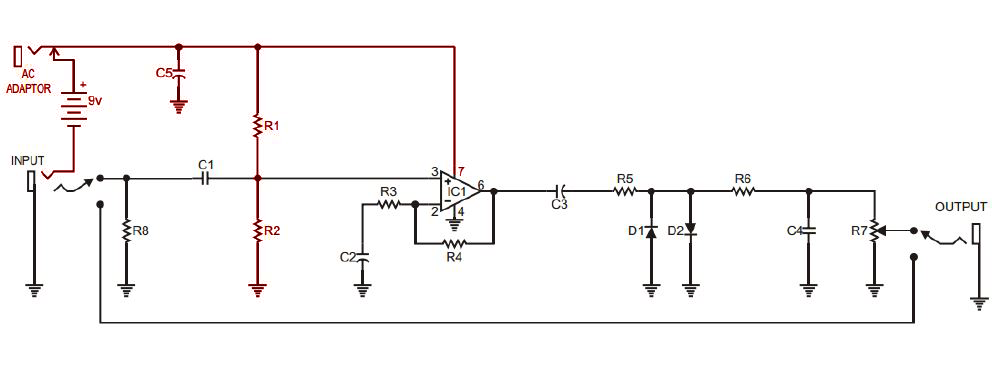
\includegraphics[width=1\textwidth, trim={0 0 0 0}, clip]{Ejercicio5/Imagenes/Circuito_base/circuito_base_alimentacion.png}
	\caption{Alimentación del circuito base.}
	\label{fig:circuito_base_alimentacion}
\end{figure}

Luego pueden verse dos resistencias $R_1$ y $R_2$, donde $R_1$ está conectada a la señal de entrada y $R_2$ está conectada a la resistencia anterior y a tierra. Este par puede considerarse de manera aproximada como un divisor resistivo, ya que en el punto medio se ofrece gran impedancia por parte tanto del op-amp (despreciando la corriente de entrada) como por el capacitor $C_1$, ya que la tensión de alimentación es constante.
Este divisor resistivo lo que está haciendo es montando a la señal de entrada sobre la tensión en el punto medio. Es en este punto donde se soluciona el problema de tener una sola fuente no partida ya que, si se cumple que $R_1=R_2$, la señal de entrada quedará levantada $4.5V$, por lo que se podría alimentar al op-amp solo de manera positiva, llevando a tierra la alimentación negativa.\\

Por último, se llevan los $9V$ de la fuente de alimentación a la entrada de alimentación positiva del op-amp.


\subsubsection{Etapa de Pre-amplificación}

\begin{figure}[H]
	\centering
	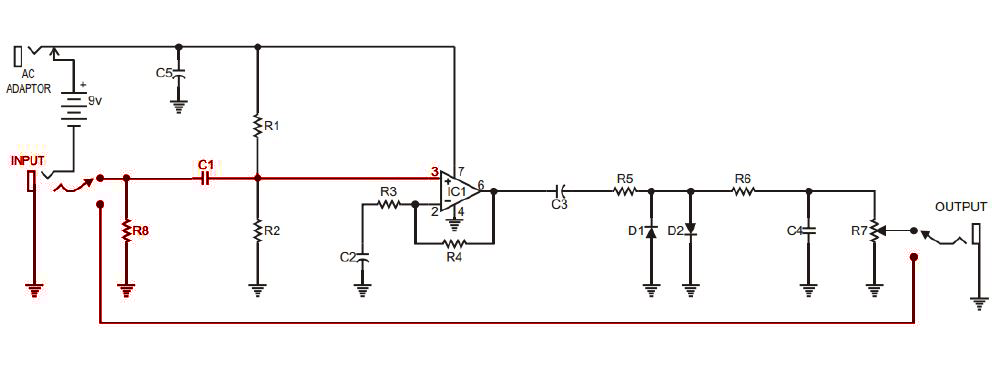
\includegraphics[width=1\textwidth, trim={0 0 0 0}, clip]{Ejercicio5/Imagenes/Circuito_base/circuito_base_preamplificacion.png}
	\caption{Etapa de pre-amplificación del circuito base.}
	\label{fig:circuito_base_preamplificacion}
\end{figure}

Justo luego de la entrada se encuentra la resistencia $R_8$. Investigando sobre posibles aplicaciones de este componente en el circuito, se llegó a la conclusión de que este resistor es utilizado para evitar un ruido de "pop" al conectar la pedalera. \textbf{Preguntar a joaco} \\

El capacitor $C_1$, como ya dicho antes, ofrece gran impedancia a la tensión continua de la alimentación para proteger a la entrada. De otra manera, la señal continua ingresaría por la entrada.
Lo que se obtiene posterior al capacitor será la señal de entrada levantada tantos voltios como proporcionen el punto medio del divisor resistivo.\\

Se contempla además que el circuito base nos permite tener una opción de realizar un bypass total al circuito mediante el uso de una llave.

\subsubsection{Etapa de Amplificación}

El operacional se encuentra realimentado negativamente con una configuración no inversora. No es un problema que no este alimentado negativamente, ya que la señal de entrada estará montada sobre una continua.

\begin{figure}[H]
	\centering
	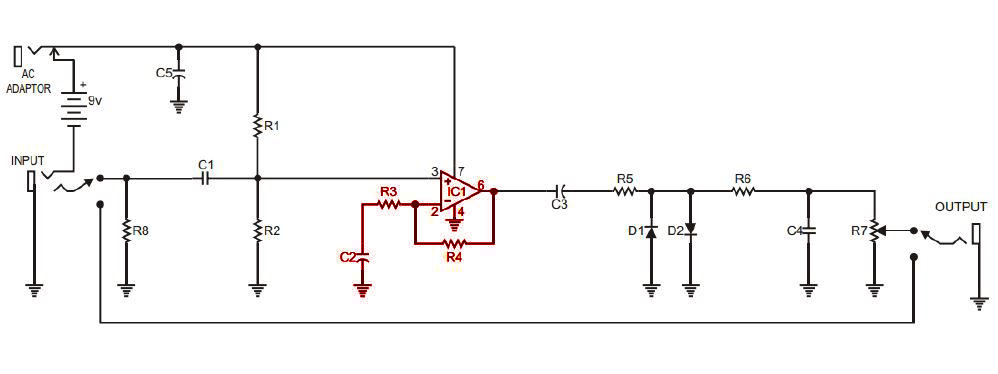
\includegraphics[width=1\textwidth, trim={0 0 0 0}, clip]{Ejercicio5/Imagenes/Circuito_base/circuito_base_amplificacion.png}
	\caption{Etapa de amplificación del circuito base.}
	\label{fig:circuito_base_amplificacion}
\end{figure}

Analizando el lazo del op-amp, se puede observar que la realimentación dependerá de la frecuencia. Esto puede observarse ya que para bajas frecuencias el capacitor actúa con gran impedancia, por lo que el operacional amplifica menos. Para las frecuencias altas el operacional amplificará cada vez más la señal hasta llegar al polo dominante. Sin embargo, lo mas importante del posicionamiento de este capacitor en el lazo de realimentación es que impide que el operacional amplifique la continua sobre la cual está montada la señal, ya que en este caso el capacitor se comporta como un circuito abierto. Esto hace que el operacional funcione como un seguidor de tensión, trabajando para fijar la continua de la salida en el mismo valor que la de la referencia. Se observa como es aquí, en el lazo de realimentación, donde se podría controlar la amplificacion de las distintas frecuencias por separado.

\subsubsection{Etapa de Ecualización}

A la salida del operacional se encuentra el capacitor $C_3$. Este capacitor se utiliza para remover la continua sobre la cual estaba montada la señal de entrada.

\begin{figure}[H]
	\centering
	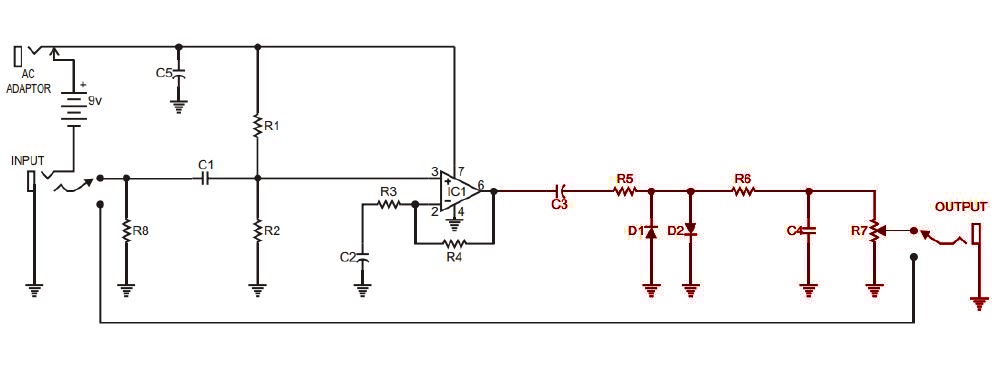
\includegraphics[width=1\textwidth, trim={0 0 0 0}, clip]{Ejercicio5/Imagenes/Circuito_base/circuito_base_ecualizacion.png}
	\caption{Etapa de ecualización del circuito base.}
	\label{fig:circuito_base_ecualizacion}
\end{figure}

Luego, se encuentra en el circuito una resistencia en serie con un par de diodos en paralelo con polaridad invertida. Estos diodos fijarían la tensión de la señal en $V_{d_{on}}$ tanto para el semi-ciclo positivo como para el negativo, deformando la señal generando un efecto de "clipping". La resistencia $R_5$ limita la corriente de los diodos. Se presume que esto se apreciaría como una gran distorsión a la hora de conectar una guitarra y escuchar la salida.\\

Seguido de los diodos se puede encontrar un pequeño circuito R-C cuya finalidad podría ser la de darle un último cambio a la señal. Este circuito estaría posicionando un polo en la respuesta en frecuencia, atenuando las frecuencias altas. Se deberá comprobar mediante simulaciones y protobordeado el posible uso de este último tramo.

Finalmente antes de la salida se encuentra un potenciómetro, el cual se presume que se utiliza como control de volumen de salida.

\subsection{Análisis Cuantitativo del Circuito Base}

Tanto el análisis cuantitativo como el subsiguiente diseño de un nuevo circuito propuesto se harán a partir de lo estudiado en tanto diversas fuentes de internet, como en el libro \textbf{PREGUNTAR NOMBRE DEL LIBRO DE AGUSTIN}.

Además, se decidió, para presentar lo realizado de la forma más clara, primero realizar un análisis teórico-analítico del circuito base para luego presentar sólamente los cambios propuestos.

\subsubsection{Componentes}

\textbf{$R_8$:} Se quiere que la impedancia de entrada al circuito sea mucho más grande que la impedancia de salida de una guitarra eléctrica con pick-ups normales, la cual es de aproximadamente $10 \ k\Omega$. Si la impedancia de entrada al circuito fuese del orden de la impedancia de salida de la guitarra, se cargarían los pick-ups y habría un desplazamiento de las frecuencias de resonancia y pérdida de agudos. Por esta razón, se decidió utilizar un valor de $2 \ M\Omega$ para este resistor. Luego en la sección de impedancia de entrada se repasara su efecto. \\

\textbf{$R_1$, $R_2$:} Se quiere montar a la señal de entrada sobre una continua de la mitad del valor que la de la alimentación, por esto, se decidió que $R_1=R_2$.

Se utilizaron valores relativamente grandes para las resistencias del divisor de tensión por dos razones:
\begin{itemize}
\item Que la corriente de stand-by no sea muy alta.
\item Contribuir a la impedancia de entrada total del circuito.
\end{itemize}
El valor utilizado es de $R_1=R_2=1 \ M\Omega$.\\

\textbf{$C_1$:} Como este capacitor filtra la continua provista por la alimentación, se decidió utilizar un valor de $15 \ nF$ ya que se quiso que el efecto del filtro pasa-altos que se forma con la resistencia $R_2$ se minimizara dentro de las frecuencias audibles ($20Hz-20kHz$).
\[ C_1=\frac{1}{2\pi R_2 f_c} = \frac{1}{2\pi 510k\Omega 20Hz} = 15.61nF \approx 15nF\]

\textbf{$C_5$:} Este capacitor filtrará el ruido proveniente de la alimentación, por lo que se eligió un valor de $33\mu F$ para presentar baja impedancia al ruido de línea de $50Hz$.
\[C_5 = \frac{1}{2\pi f X_c} = \frac{1}{2\pi 50Hz 100\Omega} = 31,8\mu F \approx 33\mu F\]

\textbf{$R_4, R_3$:} Se eligieron valores de $R_4=50R_3=1k$ para lograr una ganancia máxima en la etapa de amplificación de aproximadamente $34,15 \ dB$.
\[20log_{10}(1+\frac{R_4}{R_3}) = 34,15 \ dB\]
Generalmente, se tomaría un especial recaudo al seleccionar la ganancia que se quiere producir utilizando un op-amp, contrastando esta con la ganancia a lazo abierto provista por el fabricante, pero como en este caso se desea llevar al operacional fuera de sus límites de funcionamiento correcto para provocar efectos de distorsión, no se contemplaran dichas condiciones.\\

\textbf{$C_2$:} Este capacitor además de no dejar amplificar la continua maneja cuánto son amplificados los graves. Tras investigar el posible uso de este capacitor, se llegó a la conclusión de que un posible uso es de proteger al operacional de la inestabilidad, atenuando los bajos que pueden sobrecargar al operacional. Se calculó la capacidad analizando el filtro que se forma con $R_3$. Como la capacidad calculada es de $320nF$ 

\[ C_2 = \frac{1}{2\pi f_c R_3} = \frac{1}{2\pi 500Hz 1k\Omega} = 318,3nF \approx 320nF \]

\textbf{$C_3$:} Este capacitor está solamente para filtrar la continua de la salida del operacional pero como forma un pasa-altos con la impedancia equivalente de salida del circuito que aproximadamente es de $13,6$, y no se quiere que afecte este capacitor al circuito, su valor será de $1\mu F$ lo que dejaría la frecuencia de corte aproximadamente debajo de los $20Hz$ misma cuenta que para $C_1$.\\

\textbf{$R_5, R_6$:} $R_5$ está para limitar la corriente de los diodos, se eligió un valor de $6k8\Omega$. $R_6$ formará un filtro pasabajos con $C_4$, eligió nuevamente un valor de $6k8\Omega$.\\

\textbf{$C_4$:} Como este capacitor forma un pasa bajos con la resistencia $R_6$, se eligió un valor inicial de $1,5nF$ de tal manera que su frecuencia de corte se encuentre en $f_c = 15kHz$.
\[ C_4 = \frac{1}{2\pi 15kHz 6k8} = 1,56nF \approx 1,5nF\]

\textbf{$R_7$:} Este resistor será un potenciómetro logarítmico de $20k\Omega$. Logarítmico ya que de esta manera se acopla mejor a la escucha humana.\\

\textbf{$LM308$:} Se eligió el amplificador operacional $LM308$ ya que este posee excepcionalmente baja slew rate, lo que contribuye al efecto alineal de distorsión de la señal. Se utilizó un capacitor de compensación de $300pF$ como uno de los recomendados por los fabricantes. 

\subsubsection{Impedancia de Entrada}

Para un circuito con esta aplicación se quiere como ya dicho la mayor impedancia de entrada posible para no perder agudos o armónicos.
La impedancia de entrada del circuito base puede calcularse como
\[Z_{in} = (R8//(R1//R2))//Z_{in_{opamp}} = (2M\Omega // 500k\Omega)//40M\Omega \approx 400k\Omega\]

\subsubsection{Impedancia de Salida}

La impedancia de salida se quiere mantener lo mas baja posible, ya que la impedancia de un parlante común ronda los $8\Omega$.
La impedancia de salida del circuito base puede calcularse como
\[ Z_{out} = Z_{out_{opamp}} + 6k8\Omega + 6k8\Omega \approx 13k6\Omega \]

\subsection{Simulación del Circuito Base}

Se realizaron tres tipos de simulaciones diferentes para visualizar el funcionamiento del circuito.

\begin{figure}[H]
	\centering
	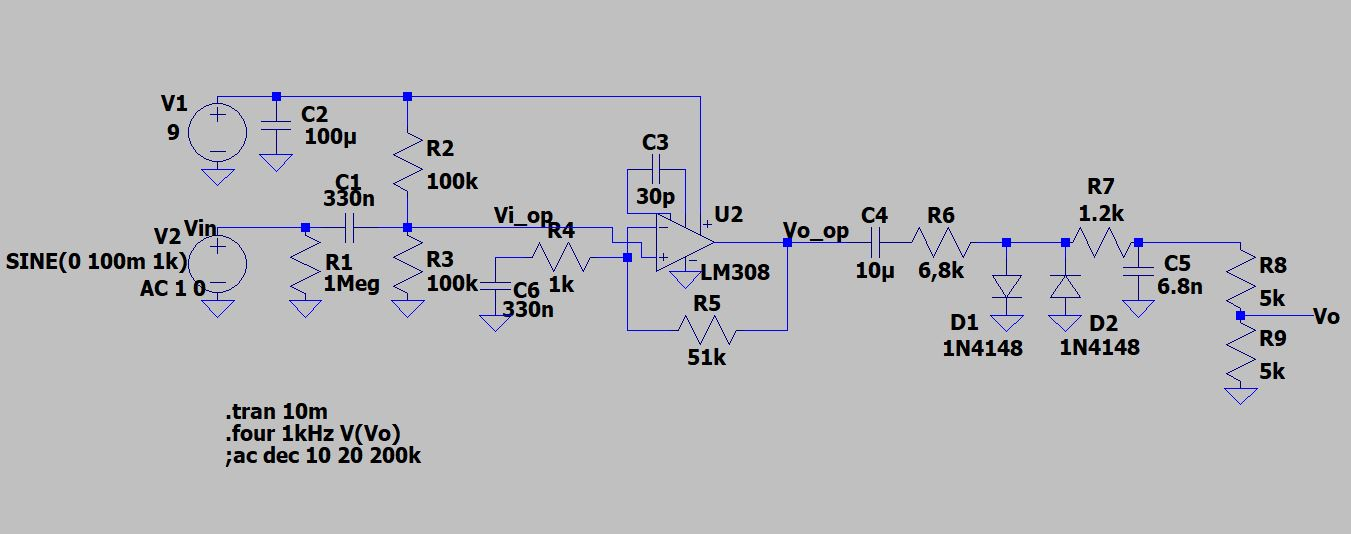
\includegraphics[width=1\textwidth, trim={0 0 0 0}, clip]{Ejercicio5/Imagenes/Circuito_base/Sim/sim_base.JPG}
	\caption{Set-up para los tres tipos de simulaciones distintas del circuito. Las dos resistencias del final emulaban un potenciómetro. Transitorio, AC-Sweep y análisis de Fourier.}
	\label{fig:sim_base}
\end{figure}

\subsubsection{Análisis de Señal, Transitorio}

Para simular el transitorio y poder observar la señal de entrada, se eligió una frecuencia media de $1kHz$ y una amplitud de $100mV$ emulando una guitarra.
Primero se analizó el accionar del divisor resistivo para comprobar la hipótesis de que este levantaría la señal de entrada por $4,5V$.
\begin{figure}[H]
	\centering
	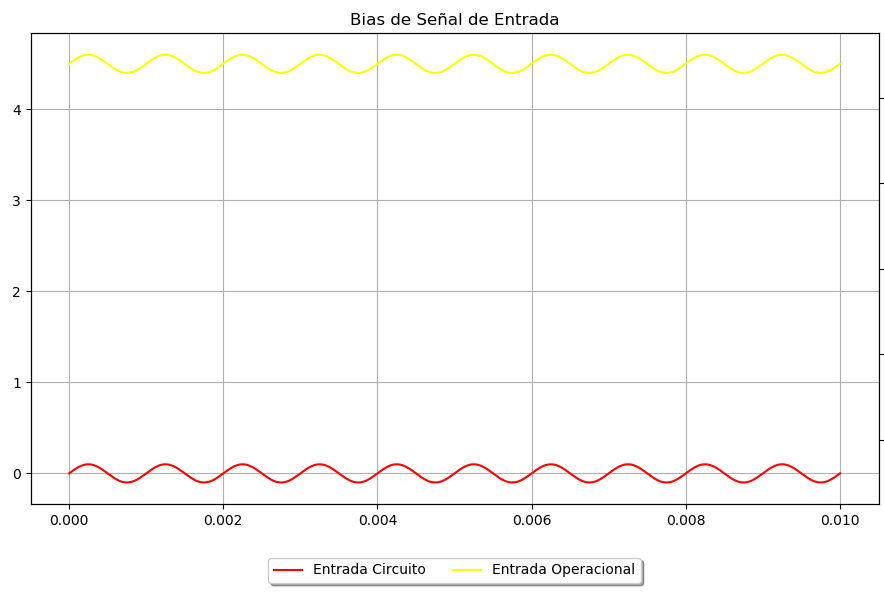
\includegraphics[width=1\textwidth, trim={0 0 0 0}, clip]{Ejercicio5/Imagenes/Circuito_base/Sim/circuito_base_tran_vi_viop.png}
	\caption{Análisis de la señal de entrada y señal de entrada al operacional.}
	\label{fig:sim_base}
\end{figure}
Se puede observar contrastando la señal de entrada con la señal que entra al opamp, que la hipótesis realizada era correcta.
Luego, se analizó la señal de salida del opamp justo antes del capacitor de acople, en contraste a la señal de entrada al operacional.
\begin{figure}[H]
	\centering
	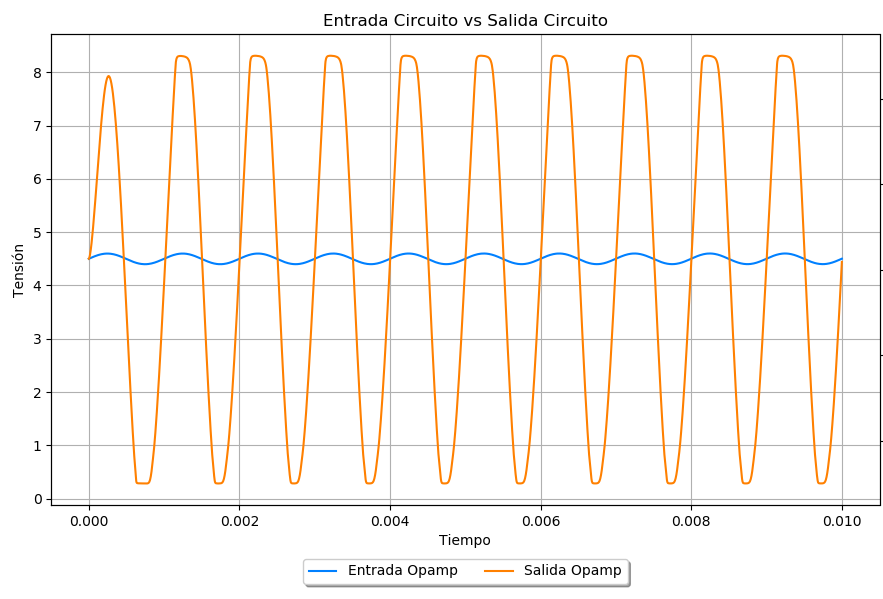
\includegraphics[width=1\textwidth, trim={0 0 0 0}, clip]{Ejercicio5/Imagenes/Circuito_base/Sim/circuito_base_tran_viop_voop.png}
	\caption{Análisis de la señal de entrada al operacional y señal de salida del operacional. }
	\label{fig:sim_base}
\end{figure}
Se puede observar como están presentes efectos distorsivos no lineales por culpa de la baja slew rate del operacional y por la saturación de este mismo, además de una gran amplificación.
Por último, se analizaron los efectos de la etapa de ecualización, contrastando la señal justo después del capacitor de acople a la salida del operacional, con la señal a la salida del circuito.

\begin{figure}[H]
	\centering
	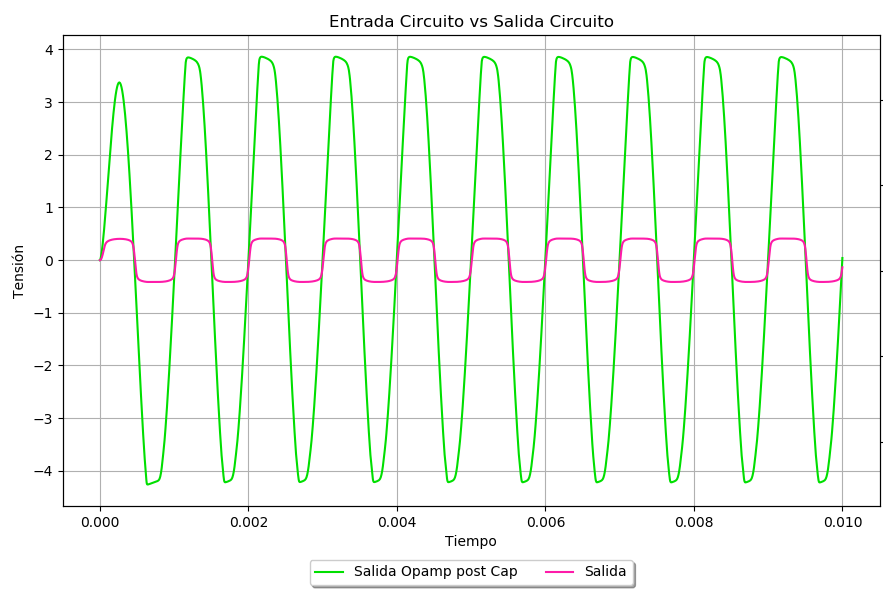
\includegraphics[width=1\textwidth, trim={0 0 0 0}, clip]{Ejercicio5/Imagenes/Circuito_base/Sim/circuito_base_tran_voop_vo.png}
	\caption{Análisis de la señal de salida del operacional luego de filtrar la continua y señal de salida del circuito.}
	\label{fig:sim_base}
\end{figure}
Se puede contemplar como la señal es recortada por los diodos, generando una gran distorsión alineal.
Finalmente, para visualizar el funcionamiento total, se contrastaron las señales de entrada y salida del circuito.
\begin{figure}[H]
	\centering
	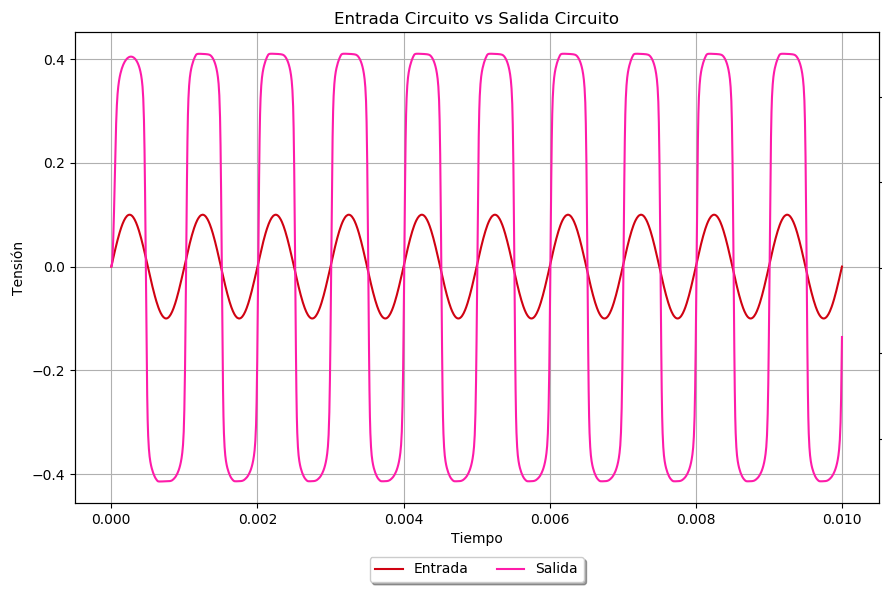
\includegraphics[width=1\textwidth, trim={0 0 0 0}, clip]{Ejercicio5/Imagenes/Circuito_base/Sim/circuito_base_tran_vi_vo.png}
	\caption{Análisis de la distorsión total en una señal de $100mV$ y $1kHz$.}
	\label{fig:sim_base}
\end{figure}
Y se puede observar el correcto funcionamiento calculado del circuito.
\subsubsection{Análisis de Bode}

\begin{figure}[H]
	\centering
	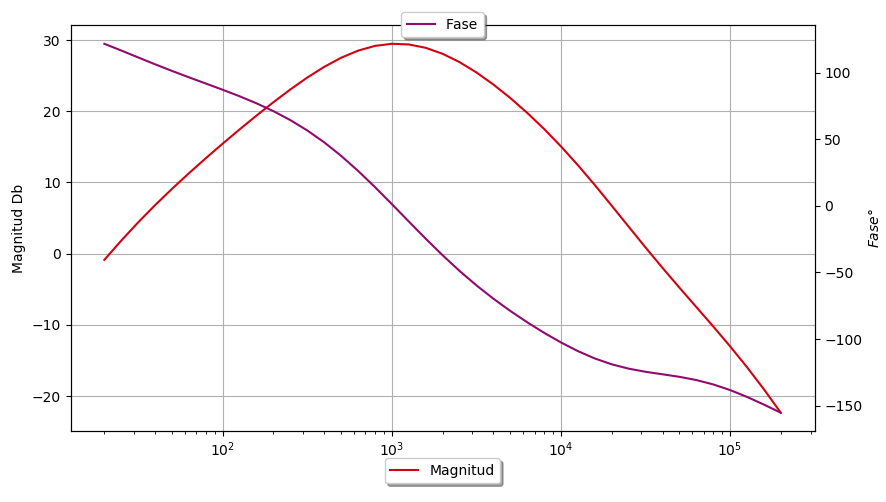
\includegraphics[width=1\textwidth, trim={0 0 0 0}, clip]{Ejercicio5/Imagenes/Circuito_base/Sim/circuito_base_bode.png}
	\caption{Gráfico de Bode para el circuito base.}
	\label{fig:sim_base}
\end{figure}

Se puede ver como hay un pico en la ganancia de $\approx 30dB$ alrededor de $1kHz$, mientras que los bajos y agudos son amplificados en menor medida.

\subsubsection{Análisis de Fourier}

Se realizó un análisis de Fourier a la salida del circuito donde se pudo comprobar que hay un $32.63\%$ de distorsión armónica a la salida, con una entrada de $1kHz$. La distorsión armónica es un parámetro para definir las señales de audio, en este caso nos está proporcionando una idea de los armónicos introducidos por la distorsión del circuito. Es calculado como el cociente entre el valor cuadrático medio de los armónicos de la señal empezando desde el segundo, y el valor del primer armónico de la señal. \textbf{Preguntar a joaco}
\begin{figure}[H]
	\centering
	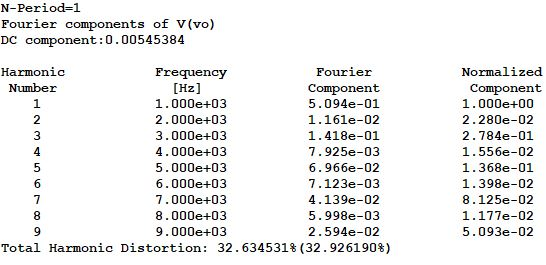
\includegraphics[width=1\textwidth, trim={0 0 0 0}, clip]{Ejercicio5/Imagenes/Circuito_base/Sim/sim_base_fourier.JPG}
	\caption{Análisis de las componentes de fourier y la distorsión armónica total.}
	\label{fig:sim_base_fourier}
\end{figure}

\subsection{Diseño propuesto}



 
\end{document}